%----------------------------------------------------------------------------------------------------------------------------------------------------------%
\PassOptionsToPackage{sorting=none}{biblatex}
%----------------------------------------------------------------------------------------------------------------------------------------------------------%
\documentclass[fontsize=12pt,twoside=semi,openright,numbers=noenddot,parskip=half]{scrbook}
\usepackage{scrhack}\usepackage{mhotext}\usepackage{geometry, graphicx, adjustbox, wrapfig, mathtools, booktabs, siunitx, setspace, subcaption, booktabs,multicol,dirtree,notoccite,xcolor,pifont}\usepackage[T1]{fontenc}\usepackage[UKenglish]{babel}\usepackage{gentium}
\usepackage{biblatex}[sorting=none,backend=biber,style=apa,citestyle=numeric-comp]\usepackage{pdfpages}\usepackage{enumitem}
\graphicspath{{./assets/}}\onehalfspacing
%----------------------------------------------------------------------------------------------------------------------------------------------------------%
\title{The Tale of a Bacteria Battle}
\subtitle{A study on Staphylococcus Aureus, its prevalence, clinical possibilities and our fighting tools}
\author{Mar Roca Cugat}
\date{Version 2.13.23}
\addbibresource{references.bib}
%----------------------------------------------------------------------------------------------------------------------------------------------------------%
\begin{document}
\maketitle
\cleardoublepage
\renewcommand{\thepage}{\arabic{page}}
%----------------------------------------------------------------------------------------------------------------------------------------------------------%
\frontmatter
%----------------------------------------------------------------------------------------------------------------------------------------------------------%
\chapter{Acknowledgements}
\begin{center}
I would like to thank Margarita Martinez, professor at the \emph{Universitat de Girona}'s Microbiology Department, as well as Olga Sánchez, professor and researcher at the \emph{Universitat Autònoma de Barcelona}'s Department of Genetics and Microbiology for their help with certain aspects of this project. \newline
I would also like to acknowledge the magnificent work that the \LaTeX\ community does to give the scientific community an incredible piece of software with which to write, as well as to Mark Olson for making his \KOMAScript\ \TeX\ template open source, allowing anyone and everyone to use it and modify it for free. On that note, I'd also like to thank my friend Gabriela, for helping me fix a weird issue with the bibliography system.\newline
But most importantly, I'd like to thank Núria Feliu, Imma Garcia and the rest of the science department for their monumental help which without this project could not have existed; as well as the subjects who volunteered to get their samples taken for this research.\newline
\end{center}
%----------------------------------------------------------------------------------------------------------------------------------------------------------%
\chapter{Ethical considerations (position TBD)}
\paragraph{}This study requires taking samples from live human subjects. This is a one-off sampling process: they are required only once. The results are then communicated to the subjects via e-mail or by being delivered a physical piece of paper. They are informed previously on the process they are going to go through, as well as the purpose of the experiment. Each subject must read and agree to two documents: an informed consent which explains everything about the experiment\footnote{Can be found at https://biblio.peiphy.xyz/TDR-IC.pdf} and a GDPR notice which documents the use of their data as well as an expected timeline for data anonymisation and destruction\footnote{Can be found at https://biblio.peiphy.xyz/GDPR-notice.pdf}. All participants were screened to be over the age of 16, in order to ease the process and require no previous authorisation by parental figures on data collection. The experimentation followed has no effect on the subjects, and they were monitored during the process in order for them not to feel any kind of stress.
\paragraph{}Since bacteria were used, some aspects of the experiment must be clarified and discussed. Previously to starting the experiment, I read profusely the WHO's Laboratory Biosafety Manual and Associated Monographs (4th Edition) as to mitigate any possible risk. During the experimentation there were 0 accidents or incidents. All plates were accounted for and controlled closely. No person other than me was allowed to come in contact with a plate that had been cultivated or with the used cotton swabs that were in the process of being disinfected. The cultivated plates were considered Biosecurity Level 2. All possibly infected material was disposed of taking into account the risks that the bacteria in question posed, using bleach.
\paragraph{}Before starting the experimentation, I had an interview with my coordinator in order to solidify the fact that there was no alternative to taking cutaneous samples from human beings, as well as a discussion on bacteria and the risks that this experiment implies.
%----------------------------------------------------------------------------------------------------------------------------------------------------------%
\chapter{Abstract}
\paragraph{}Insert abstract here
%----------------------------------------------------------------------------------------------------------------------------------------------------------%
\mainmatter\printindex\tableofcontents
%----------------------------------------------------------------------------------------------------------------------------------------------------------%
% > > > Introduction
%----------------------------------------------------------------------------------------------------------------------------------------------------------%
\chapter{Theorical context}
%----------------------------------------------------------------------------------------------------------------------------------------------------------%
\epigraph{Each source that I read, I would look through the bibliography and the footnotes, and use that as a map for the next thing I would read.}{\textit{Alexander Chee}}
%----------------------------------------------------------------------------------------------------------------------------------------------------------%
\section{Bacteria and bacterial infections}
\paragraph{Bacteria} are prokaryote organisms, generally single-celled, which are part of the Monera animal kingdom. Their sizes range from between \SI{30}{\micro\metre} and \SI{100}{\micro\metre} and are ubiquitous\footnote{Ubiquitous: found everywhere} organisms. This form of life is believed to be the first one to have ever appeared on Earth, as well as the one responsible for the oxigen-rich atmosphere the Earth currently has. Some species are hard to culture in a laboratory environment, but generally, those that can be cultured in a controlled environment are grown in agar plates\cite{murrayMicrobiologiaMedica2013}. \newline
Agar is used as a place to grow bacteria due to the fact that it is indigestible for the majority of bacteria, yet keeps them humid. Together with growth mediums, such as Lysogeny Broth, bacteria thrive in this environment, allowing them to proliferate and create colonies, which can be observed without the need of optic magnifying equipment. Sometimes, together with the growth medium, additives such as mannitol or salt are added. These are used to improve or impede bacterial growth, modify their conditions so they develop differently or as an identification tool. For example, \emph{Staphyloccus Aureus} ferments the mannitol, producing acid, which in turn generates an acid and decolorates the plate's integrated pH indicator from red to yellow, whilst the salt prevents the growth of bacteria that are not of interest to the study\cite{gamazoManualPracticoMicrobiologia2010}.
\paragraph{Pathogenic bacteria} are bacteria that have the ability to cause disease\footnote{A disease is a particular abnormal condition that negatively affects the structure or function of all or part of an organism, and that is not immediately due to any external injury\cite{DorlandsMedicalDictionary2010}.} These are not the most common type of bacteria, as the majority of them are either harmless or benefitial to the human body through symbiosis, such as the bacteria that help with digestion in the stomach\cite{murrayMicrobiologiaMedica2013}.
%----------------------------------------------------------------------------------------------------------------------------------------------------------%
\section{The enemy: \emph{Staphylococcus aureus}}
\paragraph{}\emph{Staphylococcus aureus} (also known as Staph) is a GRAM-positive bacteria, the most studied and prevalent\footnote{"The degree to which something is prevalent: the percentage of a population that is affected with a particular disease at a given time"\cite{DefinitionPREVALENCE1970}}of its genus. Staph bacteria are usually harmless. However, they can cause serious infections that, in some cases, can lead to sepsis or death. Some of its distinctive characteristics include having a very thick glycopeptide wall, which allows it to withstand extreme temperatures and osmotic pressures, therefore rendering most classic methods of food conservation (such as cooking, smoking, freezing or salting\footnote{citation needed}) completely useless against said bacteria; a protein A capsid, which binds to many eukaryote organisms; as well as thermo-resistant enterotoxins. It's an extremely resistant (and thus ubiquitous) bacteria. It can be found in human skin and mucotic surfaces (such as the mouth or the nose), as well as in certain foods such as ham (cooked or curated), eggs, raw and cooked dough, as well as in poultry.\newpage
\begin{wrapfigure}{r}{0.5\textwidth}\begin{center}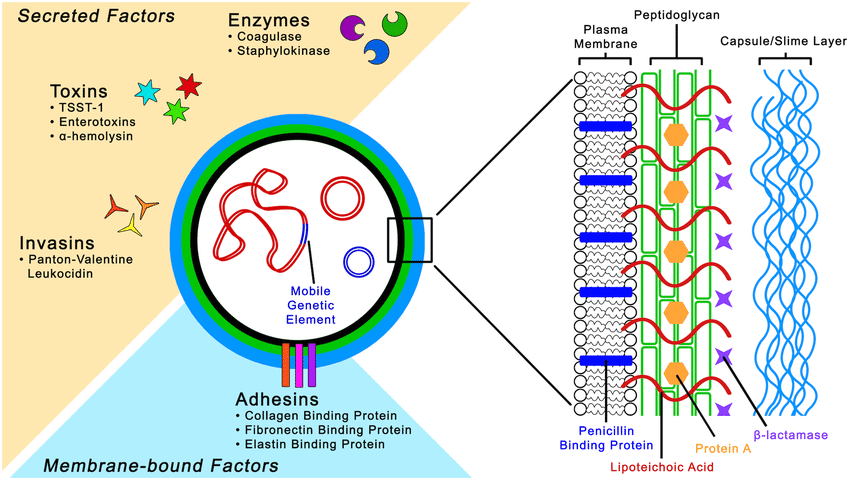
\includegraphics[width=0.48\textwidth]{staph_parts.png}\end{center}\caption{Parts of \emph{Staphylococcus aureus}. Source: PLoS Pathogens}\end{wrapfigure}\paragraph{}Staphylococcus aureus has three main parts to its virulence: its cell wall, its membrane-bound factors and its secreted factors. Staph's \textbf{cell wall} is made up of three parts, going from inside to the outside of the cell: a plasma membrane, a peptidoglycan layer and a slime (sometimes also called capsule) layer. %source: %
The plasma membrane consists of a lipid bilayer that is semipermeable\footnote{Semipermeable: it lets water and ions through, but not other molecules. This transport will always be in favour of the pressure gradient, which means that it cannot insert any kind of substance into an environment that has a higher pressure than the other side}, which regulates the transport of materials entering and exiting the cell. Integrated inside them are a type of integral protein called penicillin-binding protein (PBP), amongst other  proteins such as protein channels. We will only talk about PBPs because they are the Achilles's Heel of bacteria, as long as you know how to exploit it. Whilst the name implies PBPs are only sensible to penicillin, the name actually comes because that's how they were discovered, and in fact could be resistant to it but sensible to other antibiotic agents. Variations in this protein may lead in some cases to antibiotic resistance, such as MRSA (\emph{Methicillin-Resistant \emph{Staphylococcus aureus}}), a variation of Staph that is the result of a variation in this protein called PBP2A. The different variations of \emph{Staphylococcus aureus} will be discussed in more detail in a following section. \newline
\emph{Staphylococcus aureus}, like all other members of the \emph{Staphylococcus} family, have very thick peptidoglycan layers. This grants them protection from extreme temperatures and high osmotic pressures, which means these bacteria can colonise cooked food and food that has been salted. The most notable example is ham, either cooked, smoked or cured.
%----------------------------------------------------------------------------------------------------------------------------------------------------------%
\section{The enemy's attacks}
\paragraph{}\emph{Staphylococcus aureus} is a species that can cause a handful of different diseases, ranging from, most frequently, skin and respiratory tract infections to infective endocarditis, toxic shock syndrome or osteomyelitis. Several variations of this pathogen exist, with increasing levels of antibiotic resistance: MSSA (\emph{Methicillin-Sensitive Staphylococcus aureus}), having no resistance; MRSA (\emph{Methicillin-Resistant Staphylococcus aureus}); and VRSA (\emph{Vancomycin-Resistant \emph{Staphylococcus aureus}}), the latterthe latter for which no antibiotic concoction that can erradicate the infection is known, and the patients have to use experimental treatments. VISA (Vancomycin-intermediate \emph{Staphylococcus aureus}) is a variation that has medium resistance to vancomycin, being an intermediate step between MRSA and VRSA. VISA and VRSA are what we would call a superbug, a microbe that has developed resistance to more quantity of antibiotic than is safe to consume. Studies have discovered that this genetic factor has been developed by different lineages separetely, indicating that there is not a common ancestor of MRSA strains. This case is the bacteria equivalent of carcinisation, the discovery that several species have coevolved into crabs; as well as the bacteria equivalent of tree leaves, which were developed independently by several species at the same time, in completely different parts of the world. 
\paragraph{}One of Staph's most notorious abilities is using the body's own proteins to disguise itself and thus avoid detection and phagocytosis by the host's immune system. It accomplishes this task by using enzymes called coagulases, which enable the transformation of fibrinogen \footnote{A glycoproteic complex produced in the liver and present in the blood of all vertebrates.} to fibrin \footnote{fibrinogen after being stimulated by either thrombin or \emph{staphylothrombin}, the result of a molecular pathway stimulated by coagulase. It helps in clotting the blood in the event of vascular or tissue injury}\cite{murrayMicrobiologiaMedica2013}. Only 11 other \emph{Staphylococcus} family members are coagulase-positive. To test for this enzyme in the laboratory there are two main methods which are usually combined: culture of the sample on a Baird-Parker agar medium, a selective and differential medium which contains lithium chloride and tellurite as to inhibit the growth of other microbes. It also includes pyruvate and glycine, which promote the growth of \emph{Staphylococci} colonies, showing in colour black and with an opaque zone around the colony. This opaque zone represents the effect of the coagulase. Another way to test for coagulase is to perform a coagulase test. This test generally requires a small quantity (generally 2 mL) of sheep blood serum, which will gelatinise if coagulase is present.
\paragraph{}\emph{Staphylococcus aureus} contains an important quantity of \textbf{toxins}. which grants it most of its pathogenicity. Many of its virulence factors can be described as such. Toxins are usually defined as poisonous substances, which, in our case, means that they have the capacity to mess with the host body directly, without need of a mediating entity. This category doesn't include, for example, those molecules intended to combat the host's defence mechanisms or scavenge reactive oxygen. We'll also exclude those situated on its membrane for the purpose of cell binding. Staph has several kinds of toxin in its arsenal: membrane-damaging toxins (which can be receptor-mediated or not), receptor-interfering toxins (not membrane-damaging), enzymes, and pathway blockers.\newline
\begin{itemize}
\item[$\bullet$] Membrane-damaging toxins. Several of \emph{Staphylococcus aureus}' toxins target the cytoplasmic membrane of the host's cells. These lead to pore formation in it, which provokes the outflux of vital molecules of the cell which, in turn, leads to cytolysis\footnote{Cell bursting due to osmotic pressure imbalance between the inside and the outside of it}.
   \begin{itemize}
        \item Receptor-mediated. Many of the cytolytic toxins of \emph{Staphylococcus aureus} have been shown to require receptor interaction for their lytic activity. The best-known toxin of this kind is Alpha-toxin, also known as Alpha-hemolysin, which is its major cytotoxic agent, and is lytic to red blood cells and certain leukocytes, but not to neutrophils. Whilst at low concentrations it has been shown to be dependent on the interaction with cells' ADAM10 receptors, in higher concentrations of this toxin, this interaction is no longer necessary. Other toxins of this type include  PVL (Panton-Valentine Leucocidin) and Gamma-toxin.
        \item Non-receptor-mediated. In 2007, a toxin family that includes the Delta-toxin called the Phenol-Soluble Modulins (PSMs). PSMs trigger an inflamatory response by interacting with the FPR2 receptor, however they can carry cytolytic activity independently from FPR2 interaction. Delta-toxin has been linked to allergic skin sease and atopic dermatitis by degrading mast cells. This kind of toxin contributes to neutrophil lysis after phagocytosis, which might partly explain why the development of \emph{Staphylococcus aureus} vaccines that work by enhancing a type of phagocytosis have failed so far. 
   \end{itemize}
\item[$\bullet$] Receptor-function-interfering toxins. The toxins that fall into this category are enterotoxins\footnote{Enterotoxins are those toxins that target the intestines.} These typically cause vomit and diarrhoea. \emph{S. aureus} strains can produce a wide array (around 20) of entero and entero-like toxins. The most famous \emph{Aureus} superantigen\footnote{Superantigen: type of antigens that results in excessive activation by the immune system}, the 22-kD toxic shock syndrome toxin (TSST), belongs to this group. TSS is a very severe and potentially fatal disease. \emph{Staphylococcus aureus} also secretes a series of proteins that interfere with leukocyte receptors to evade recognition and thus activation of the immune system. CHIPS (Chemotaxis Inhibitory Protein of \emph{Staphylococcus aureus}), which binds to the C5aR and FPR receptors, impairing the recognition of bacterial formylated peptides by the FPR receiver and blocking the activation of leukocytes via C5aR. \emph{S. aureus} also has other proteins that work similarly to these, such as FLIPr.
\item[$\bullet$] Enzymes. Many enzymes secreted by \emph{Staphylococcus aureus} either degrade host molecules or interfere with its metabolic or signalling cascades. A few of them are proteases, which some non-specific ones have the ability to degrade host proteins in a broad proteins, leading to tissue destruction and necrosis, but may also have some more specific effects, for example the destruction of insulin B. Its two coagulases (staphylocoagulase and Willebrand factor) fall into this category.
\end{itemize}
%----------------------------------------------------------------------------------------------------------------------------------------------------------%
\section{Our weapons}
\paragraph{} The tools we have at our disposal to fight off this infection fall into two main categories: chemical factors and biological factors.
\paragraph{} The chemical factors are drugs, and they depend both in quantity and type on the variation a particular case falls in. It is \textbf{extremely important} to find out the level of antibiotic resistance that specific infection has before administering any antibiotic, as this treatment course will cause side effects such as killing gut bacteria, diminishing defense system capabilities, and increasing the possibility to develop yet more resistant infections. Generally, a large-spectrum antibiotic has an adequate risk-to-benefits ratio of causing the latter, so they may be used before switching to a more specific treatment.
\paragraph{}\begin{wrapfigure}{r}{0.35\textwidth}\begin{center}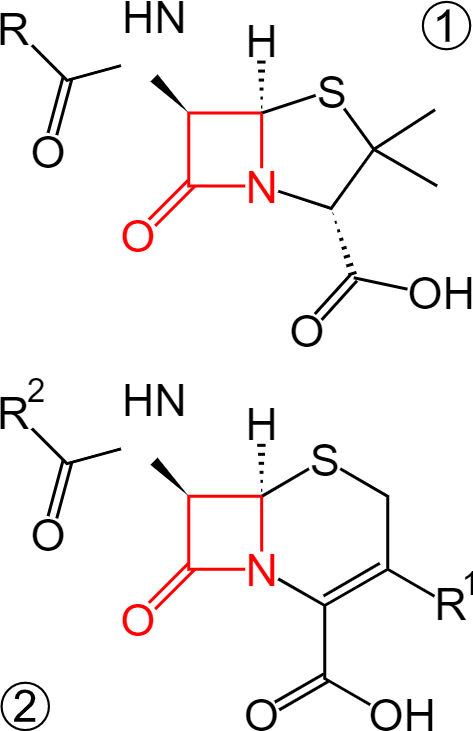
\includegraphics[width=0.30\textwidth]{assets/beta-lactam.png}\end{center}\caption{Organic chemistry structure of penicillin (top) and cephalosporin (bottom). β-lactam ring in red. Source: WikiMedia}\vspace{-0.30\linewidth}\end{wrapfigure}Starting with the treatment to the least resistant strains of \emph{Staphylococcus aureus}, a β-lactam antibiotic (such as methicillin, oxacillin, cloxacillin and penicillin) is the weapon of choice to fight against an MSSA infection. This is because this specific chemical part (just a \beta-lactam ring does nothing by itself) has the ability to inhibit cell wall biosynthesis on the bacterial intruder's body. But once the β-lactam ring is cut by an enzyme secreted by the bacteria itself, this type of antibiotic suddenly loses effect against them.
\paragraph{}That's where Vancomycin comes in. It is a type of glycopeptide antibiotic, just like \beta-lactam and works by blocking the construction of a cell wall, as all of its type do. This treatment is extremely invasive and only indicated for the treatment of extremely serious life-threatening infections by Gram-positive bacteria that have shown to be unresponsive to other antibiotics.\begin{wrapfigure}{l}{0.35\textwidth}\begin{center}
\includegraphics[width=0.30\textwidth]{assets/vancomycin.png}\end{center}\caption{Organic chemistry structure of vancomycin. Source: WikiMedia}\vspace{0.15\linewidth}\end{wrapfigure}\newline It can be taken as a pill or as an injectable fluid, which proves it to be much more effective. This treatment is incompatible with aminoglycosides, a type of antibiotic that inhibit protein synthesis, as it can lead to nephrotoxicity\footnote{Nephrotoxicity: damage to the kidneys} and ototoxicity\footnote{Ototoxicity: damage to hearing}. Vancomycin can induce platelet-reactive antibodies in the patient, leading to severe thrombocytopenia and bleeding with petechial hemorrhages on the tongue and bruises. Unfortunately, even with use of Vancomycin, Staphylococcus aureus can develop resistance. In this case, no other option than using a biological factor is left. There has been one study in 2020 that discovered that by modifying the bacteria with a cationic oligopeptide\footnote{Cationic oligopeptide: sequence of two or more aminoacids that is positively charged}, vancomycine resistance could be bypassed. This could be a good solution temporarily as we wait for phage therapy to get approved, if it was a sufficiently studied option, which is not. This was discovered in 2020, while bacteriophage trials have been ongoing since the mid 2000s.
\paragraph{}The biological factor is a bacteriophage, called P68. It comes from the \emph{Caudovirales} order, which means that it is a bacteriophage with tail.  This treatment is still in testing, but it appears to be effective and lead to low adverse results. If possible, it would be preferrable to use bacteriophage therapy (shortened to phage therapy) instead of going for antibiotics, as can lead to less side effects than antibiotics, as it only attacks a specific bacteria. This means, unfortunately, that the infection has to be pinpointed with extreme accuracy. The use of this treatment also negates the risk of bacteria developing antibiotic resistance. It is, however, unclear whether the bacteriophage could mutate into a dangerous strain. This class of virii has been studied since the late 19th century after being discovered by accident in water from a river in India. This research, however, was dropped due to penicillin being discovered and put into effect, as the main purpose of this research was to use it on war casualties as to reduce mortality due to infections.
\newpage{}\begin{wrapfigure}{r}{0.35\textwidth}\begin{center}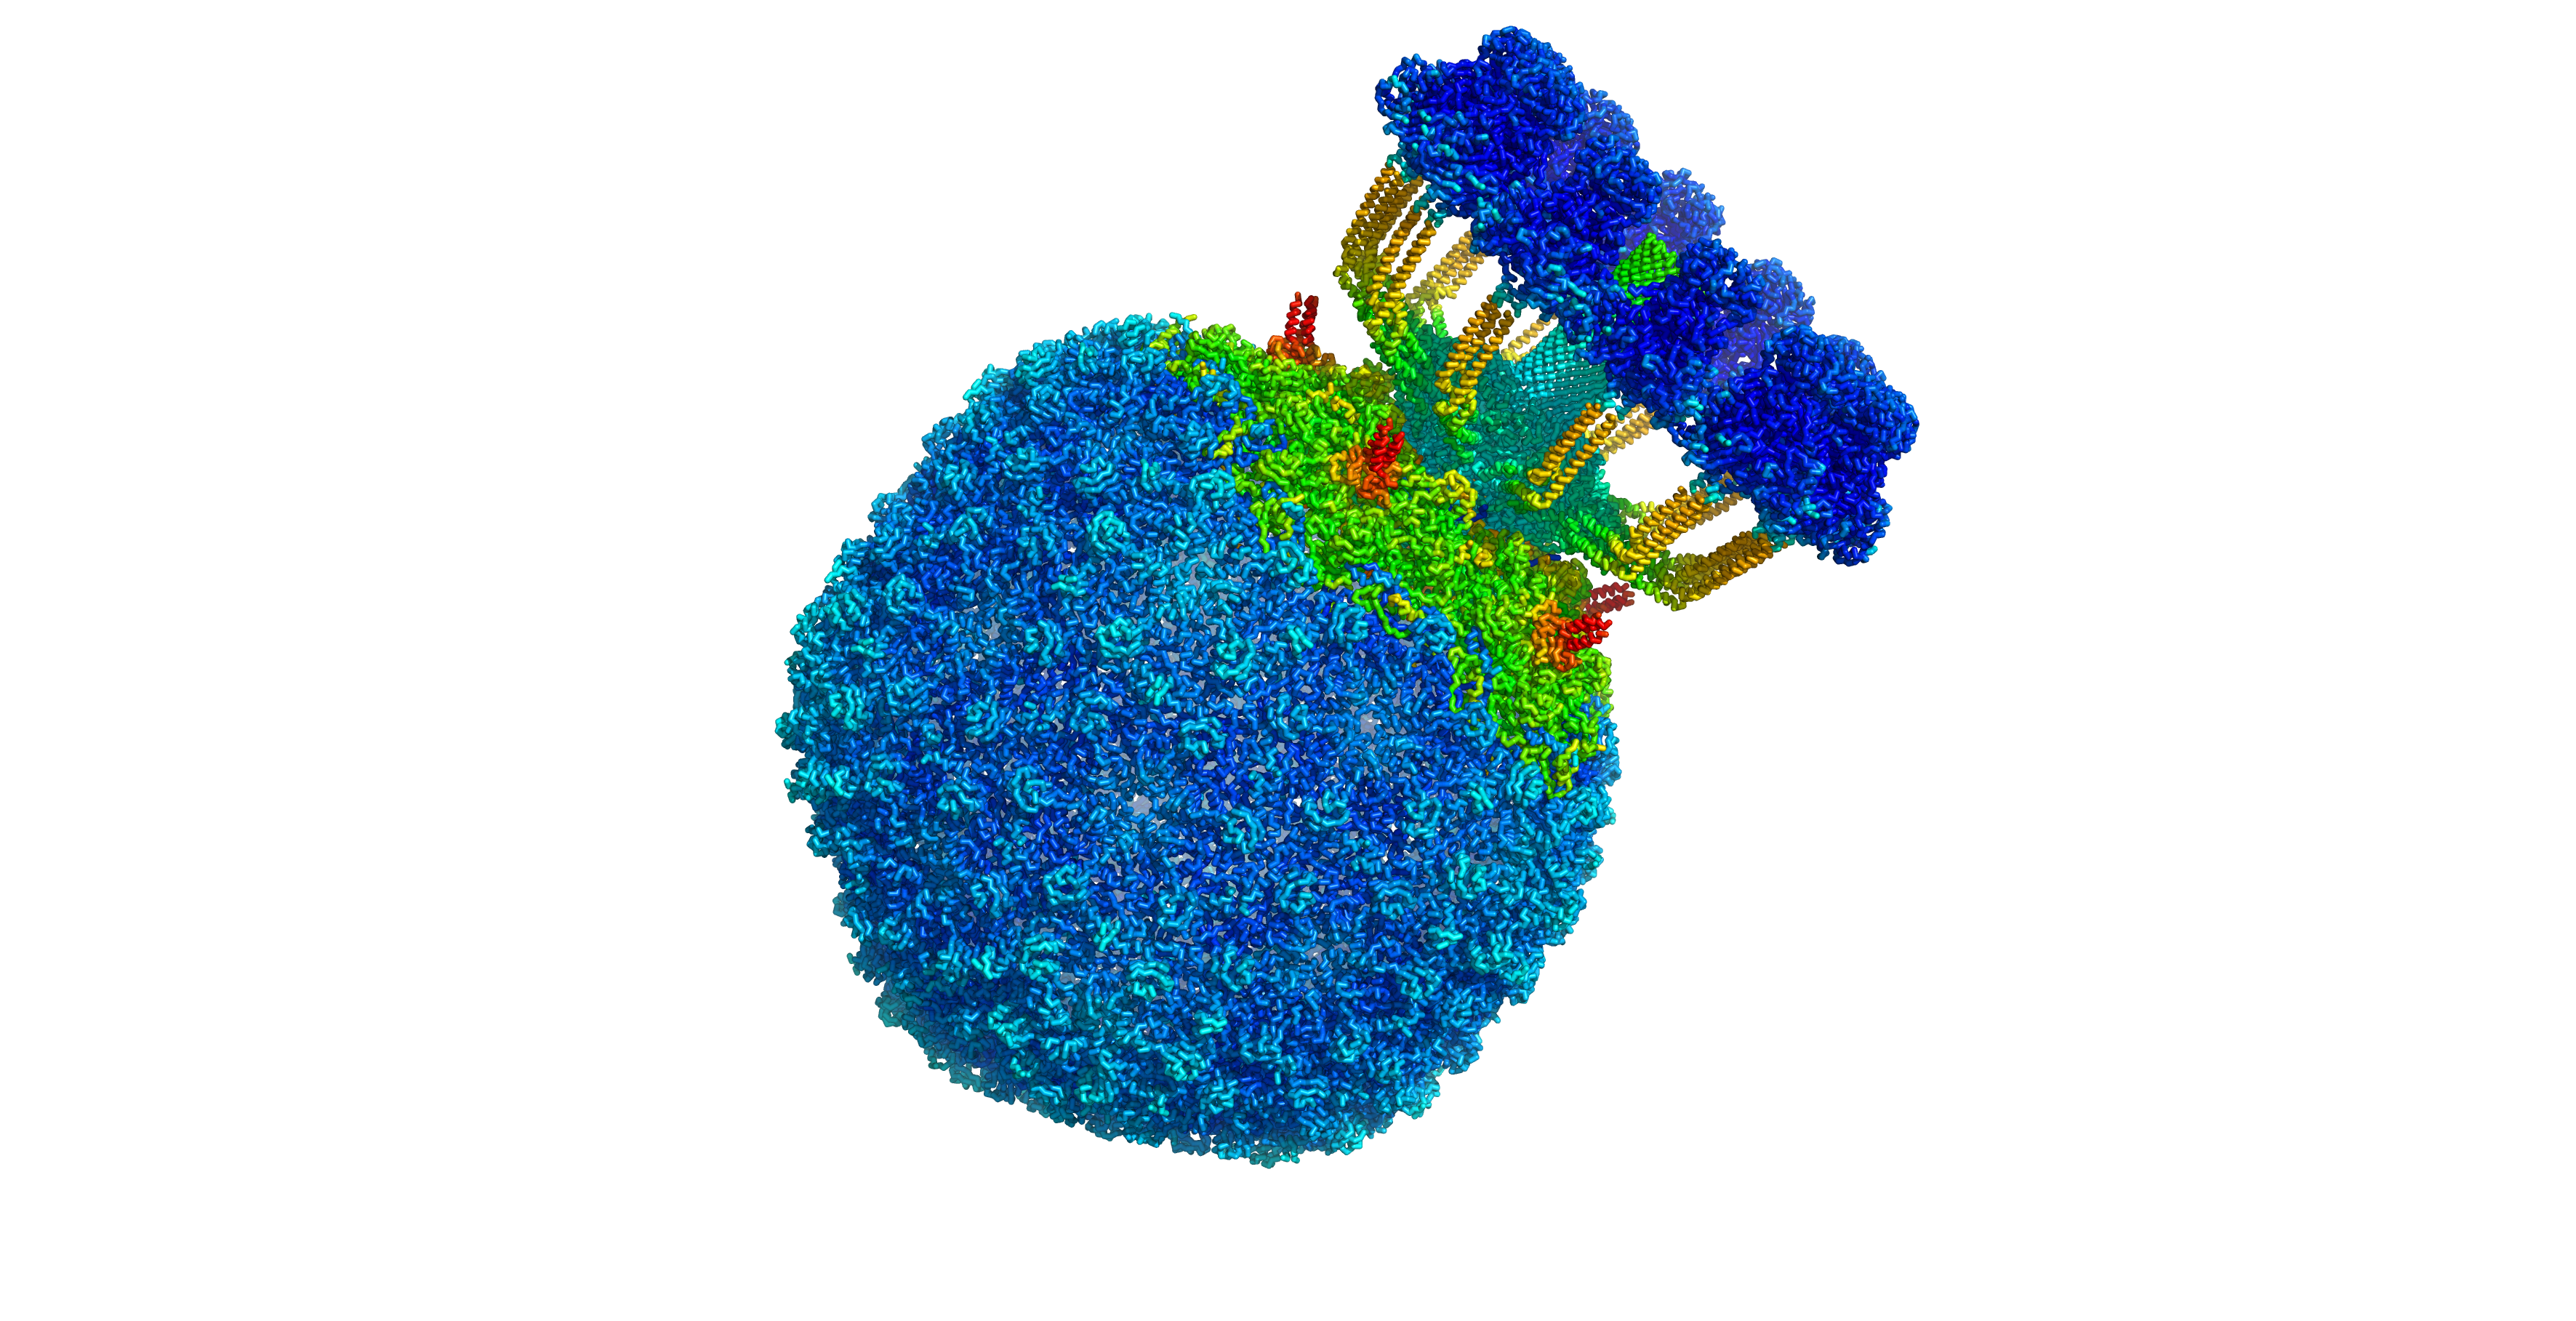
\includegraphics[width=0.30\textwidth]{assets/staph_side.png}\end{center}\caption{P68 structure. Source: Own results}\end{wrapfigure}Bacteriophages work in an interesting manner. They work by detecting one very specific bacteria, just like any other virus does with the type of cell they evolved for, then bind to it and inject their genetic material, which then in turn the bacteria considers as its own, inserts it into its own genetic sequence and starts producing the proteins the virus requires, but it doesn't eject them. Once the bacteria is full with phages, a special lytic compound is released which bursts the cell membrane in such a way that it resembles an explosion, but instead of heating up everything in a radius, spreads millions more of bacteriophages, which then bind to other bacteria and the cycle repeats until there's no more bacteria left. The fight from the bacteria point of view consists mostly on trying to outnumber and outreproduce the phages as to have a chace of survival, even if minimal. There is no known bacteria that shows resistance to phages. That is probably because unlike the chemical factors, phages can evolve and improve with each generation.
%----------------------------------------------------------------------------------------------------------------------------------------------------------%
\section{Ethical considerations}
\paragraph{}This study requires taking samples from live human subjects. This is a one-off sampling process: they are required only once. The results are then communicated to the subjects via e-mail or by being delivered a physical piece of paper. They are informed previously on the process they are going to go through, as well as the purpose of the experiment. Each subject must read and agree to two documents: an informed consent which explains everything about the experiment\footnote{Can be found at https://biblio.peiphy.xyz/TDR-IC.pdf} and a GDPR notice which documents the use of their data as well as an expected timeline for data anonymisation and destruction\footnote{Can be found at https://biblio.peiphy.xyz/GDPR-notice.pdf}. All participants were screened to be over the age of 16, in order to ease the process and require no previous authorisation by parental figures on data collection. The experimentation followed has no effect on the subjects, and they were monitored during the process in order for them not to feel any kind of stress.
\paragraph{}Since bacteria were used, some aspects of the experiment must be clarified and discussed. Previously to starting the experiment, I read profusely the WHO's Laboratory Biosafety Manual and Associated Monographs (4th Edition)\cite{worldhealthorganizationLaboratoryBiosafetyManual2020} as to find ways to mitigate any possible risk. During the experimentation there were 0 accidents or incidents. All plates were accounted for and controlled closely. No person other than me was allowed to come in contact with a plate that had been cultivated or with the used cotton swabs that were in the process of being disinfected. The cultivated plates were considered Biosecurity Level 2. All possibly infected material was disposed of taking into account the risks that the bacteria in question posed, using bleach.
\paragraph{}Before starting the experimentation, I had an interview with my coordinator in order to solidify the fact that there was no alternative to taking cutaneous samples from human beings, as well as a discussion on bacteria and the risks that this experiment implies.
% > > > Experimental, round 1
%----------------------------------------------------------------------------------------------------------------------------------------------------------%
\chapter{Physical experimentation}
\epigraph{A scientist in his laboratory is not a mere technician: he is also a child confronting natural phenomena that impress him as though they were fairy tales.}{\textit{Marie Curie}}
%----------------------------------------------------------------------------------------------------------------------------------------------------------%
\section{Description}
\paragraph{}This experiment is designed to detect and evaluate the prevalence of \emph{Staphylococcus aureus} in a sample of students from our school. The process used involves extracting a sample from underneath a subject's nails by swabbing, cultivating that sample, and then observing the results of said culture to determine the presence or not of \emph{Staphylococcus aureus} as part of the subject's resident bacterial flora. Each sampling iteration of the process took less than two minutes to complete. However, all the safety measures and actions taken need more time to be taken care of properly; as well as taking into account the fact that cultivating is not a task that can be done in just a day, often needing two to three to fully develop.
%----------------------------------------------------------------------------------------------------------------------------------------------------------%
\section{Protocol followed}
\paragraph{}The protocol followed was designed based on a similar protocol used in many university laboratories\cite{olearyPracticalHandbookMicrobiology1989}, modified to fit the needs of this research paper, peer-reviewed by Olga Sánchez, and uploaded to the Protocols.io platform, to make it easier to follow the days of that the experiment took place in. This protocol underwent 10 different revisions\cite{rocacugatStaphilococcusAureusSampling2022a}. It dictates the following steps: \newline\begin{wrapfigure}{r}{0.4\textwidth}\begin{center}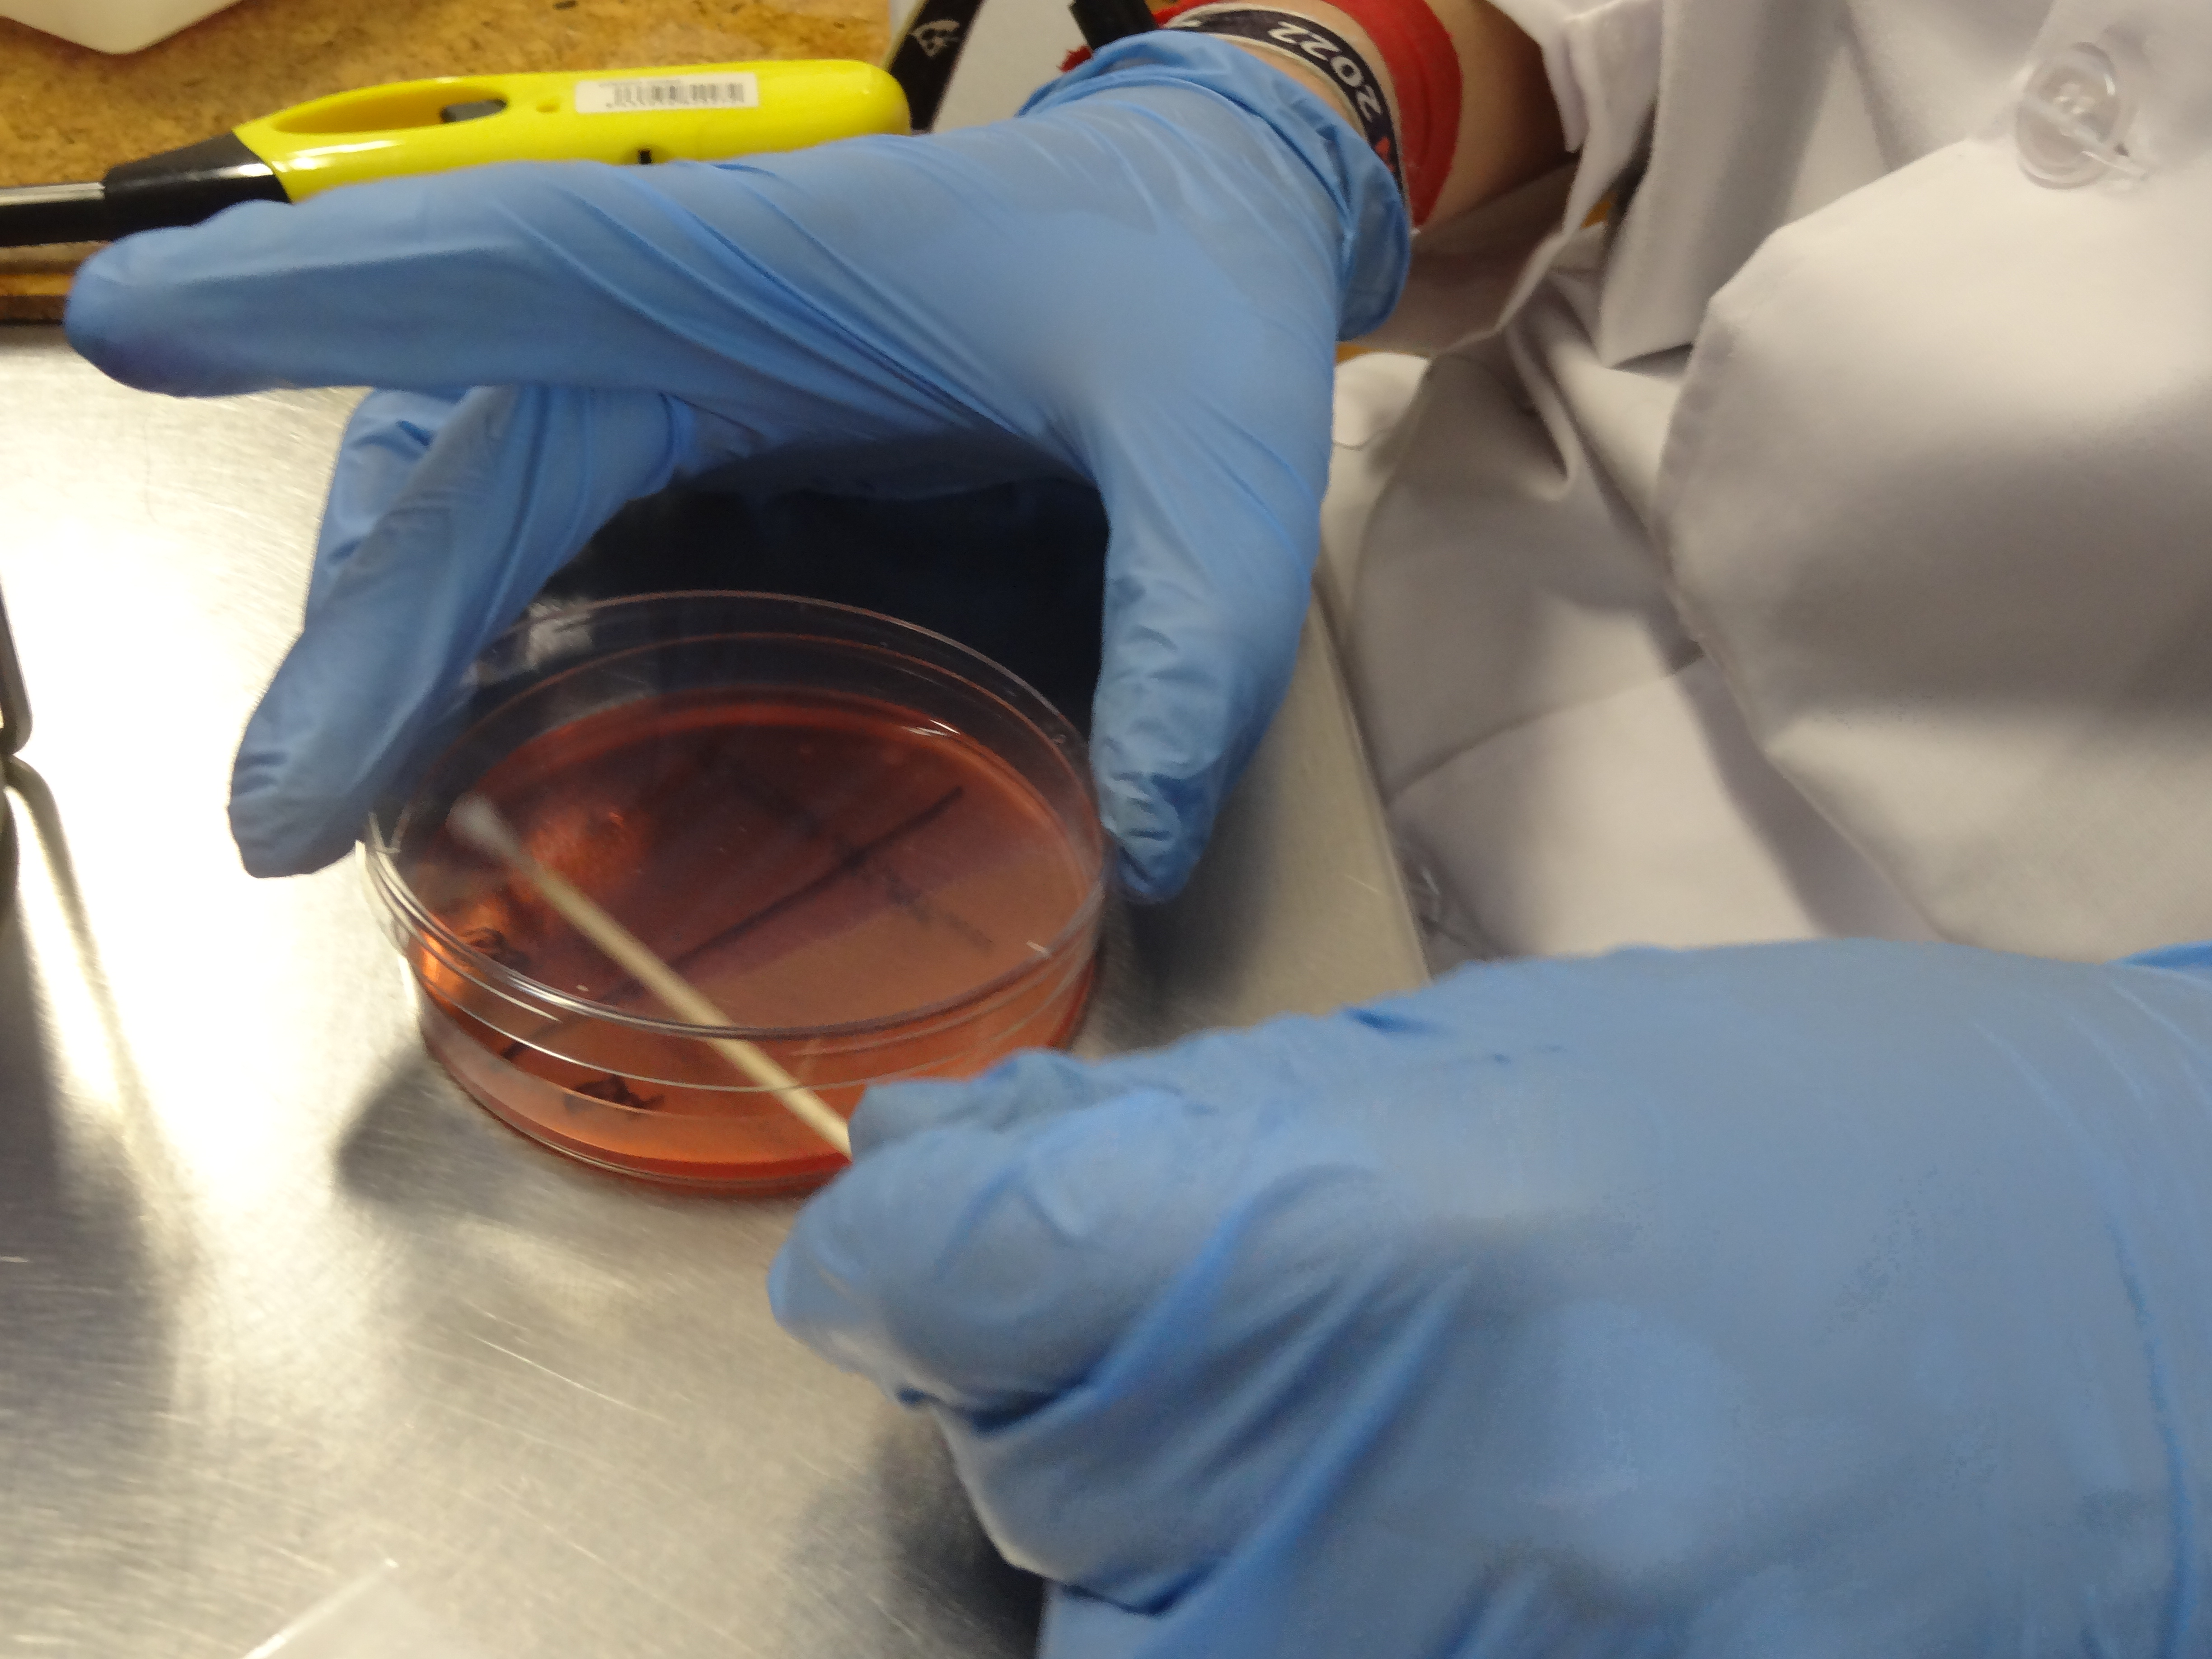
\includegraphics[width=0.38\textwidth]{sampling.JPG}\end{center}\caption{Transferring a sample to the agar plate}\end{wrapfigure}
\begin{enumerate}[label=\arabic*)]
\item Prepare yourself for the experimentation: wash your hands, put on gloves, put on the lab coat, mask, and goggles. Wash your hands again (gloves still on). Set up the work area; the Bunsen burner should be turned on in such a way that it can cover an acceptable surface to work. Turn it on and try not to break sterility\footnote
\item Divide each Petri dish in 2 parts. A ruler should be used for this part. Get your subject to wash their hands and observe them. If the nails are extremely short, it may be worth it to take the sample nasally. If the hands don't seem clean enough, teach them proper hand washing techniques.
\item Note down their information, crack open a sterile swab pack, dip one of the swabs in Ringer solution and swab away at under their nails or nose. Then, populate the dish with this sample.
\item Incubate for 32-48h and observe the results.
\item Observe the bacteria under a microscope after a GRAM tinction.
\end{enumerate}\newpage
%----------------------------------------------------------------------------------------------------------------------------------------------------------%
\section{Bill of materials}
\paragraph{}The materials used, as well as the quantities used, can be found in the following table. On the left, laboratory equipment and, on the right, reagents, tinction agents, and consumables used:
\begin{center}\begin{figure}[H]\centering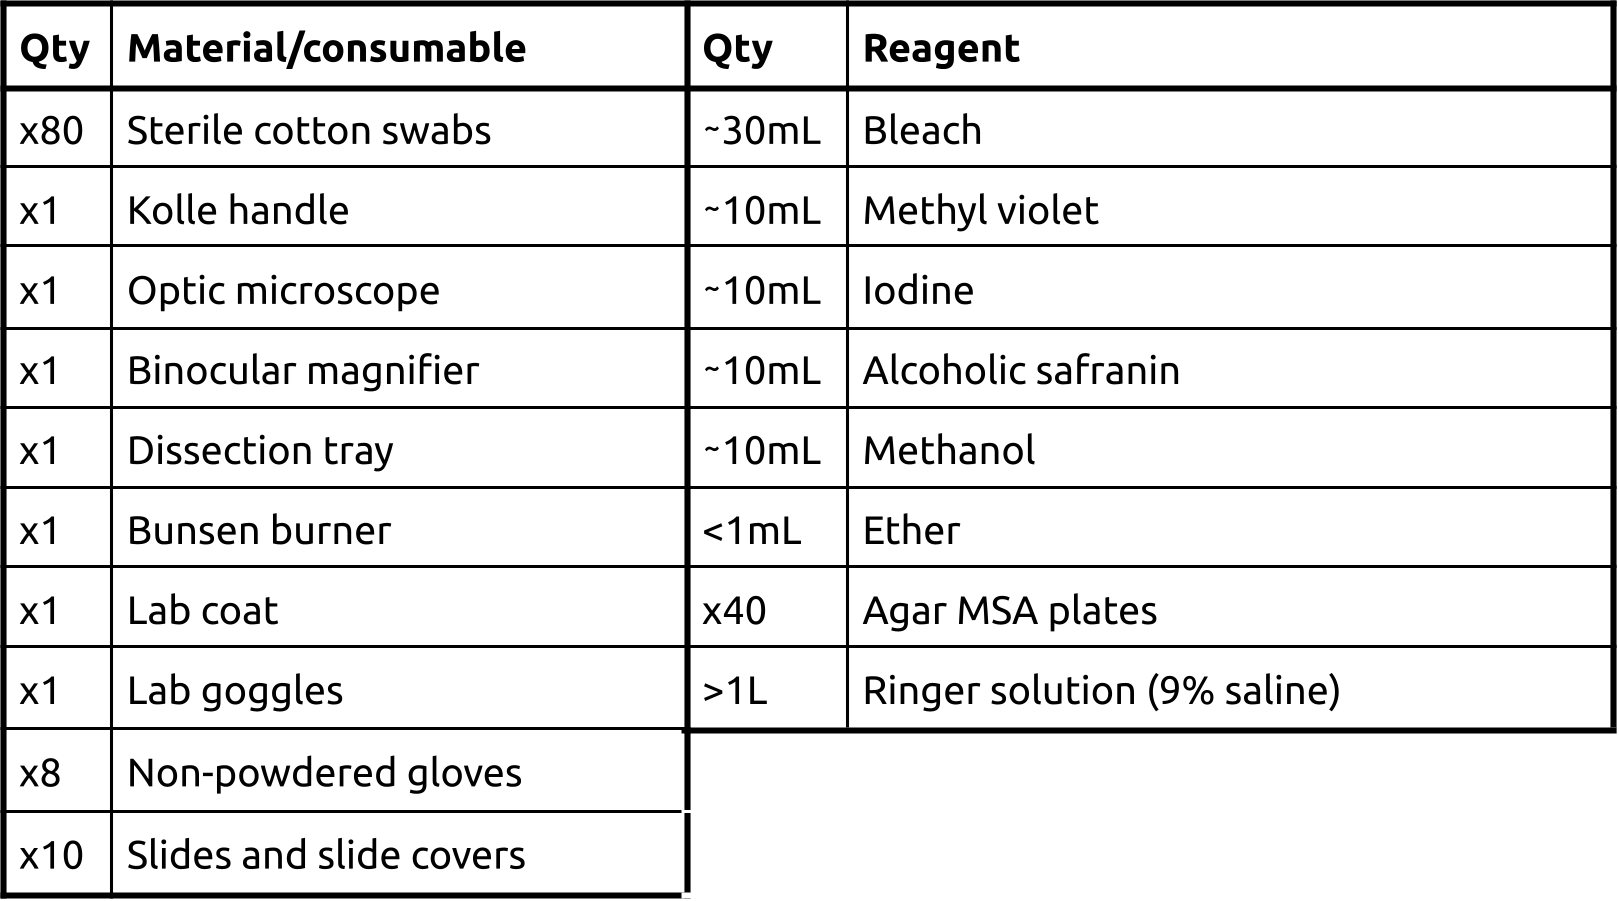
\includegraphics[width=0.90\textwidth]{BOM-1.png}\end{figure}\end{center}
%----------------------------------------------------------------------------------------------------------------------------------------------------------%
\section{Biosecurity and risk mitigation}
\paragraph{}Staph is considered a Biosecurity Level (BSL) 2 pathogenic bacteria\cite{cheungPathogenicityVirulenceStaphylococcus2021}. This means that it is associated with a human disease that can pose a moderate human health hazard. In a laboratory where BSL-2 pathogens are handled, usual lab rules should be followed (mechanical pipetting only, surgical hand-washing, prohibition of the consumption of food and drinks in the lab, proper PPE use… as well as avoiding splashes or aerosols, adhering biohazard warning signs present on all material used, as well as proper surface and material disinfection via the use of autoclave or proper alternative decontamination method.\newline
The risks associated with this bacterium were assessed following the protocol designated by the World Health Organisation, and proper security measures were followed at all times when handling biohazardous material. No incidents occurred during the research part of this project, and the protocol defined previous to the start was followed extremely closely. While the laboratory used may not be the most ideal type of laboratory for this type of research, it was certainly adequate to perform a research project like this one, especially after the temporary signage that was temporarily installed\cite{worldhealthorganizationLaboratoryBiosafetyManual2020}.\newpage
%----------------------------------------------------------------------------------------------------------------------------------------------------------%
\section{Results and analysis}
The results obtained can be found in the following raw data table:
\begin{center}\begin{figure}[H]\centering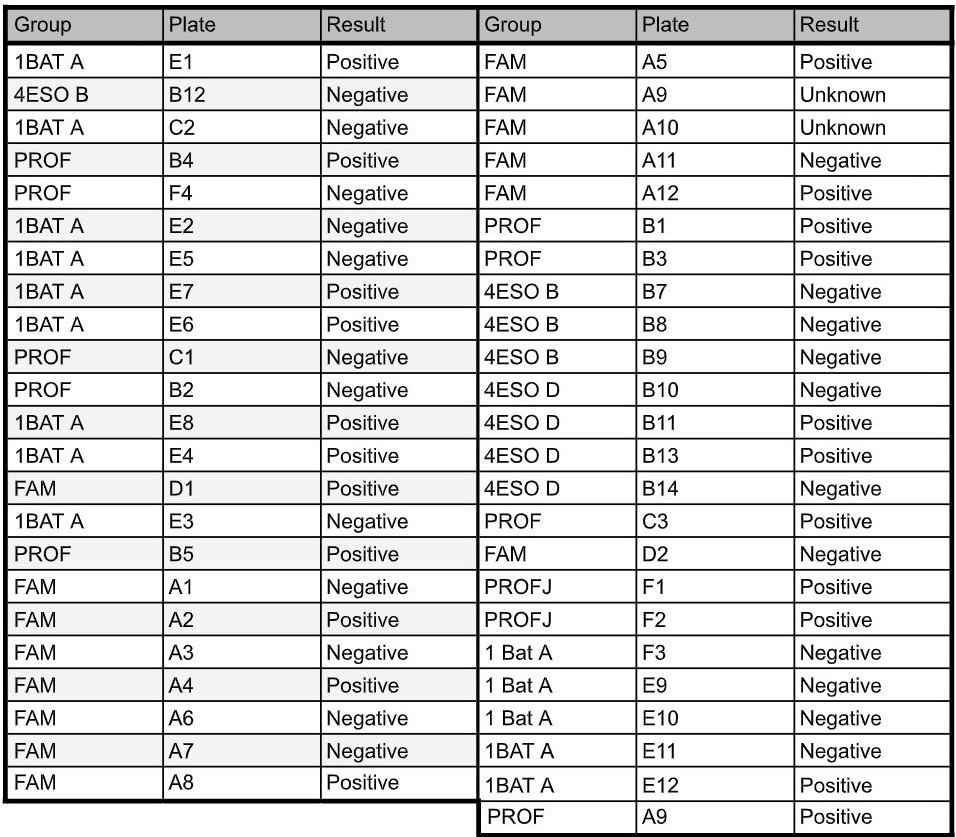
\includegraphics[width=0.80\textwidth]{RES-1.jpg}\end{figure}\end{center}
The data was then recounted and graphed into the following pie chart:
\begin{center}\begin{figure}[H]\centering\begin{subfigure}[b]{0.4\linewidth}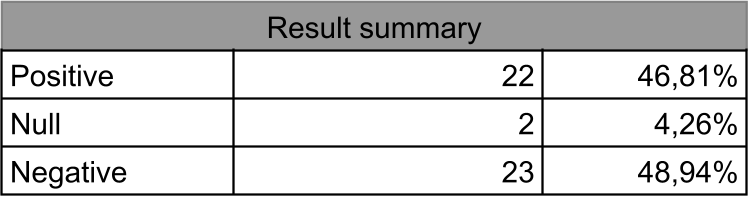
\includegraphics[width=0.95\linewidth]{Data.png}\caption{Counts of the result cases.}\end{subfigure}\begin{subfigure}[b]{0.38\linewidth}\includegraphics[width=0.95\linewidth]{Pie.png}\caption{Pie graph of the result cases.}\end{subfigure}\caption{Data processed from results}\end{figure}\end{center}\vspace{-1.5em}
As we can see, almost 50\% of the samples taken tested positive for \emph{Staphylococcus aureus}, compared to the expected 30\%\cite{StaphylococcusAureusHealthcare2020}. We can, however, see in the UK's Public Health bactaeremia data that Staph infections have been on the rise lately, so it may not be a case of wrong data\cite{englandMSSABacteraemiaAnnual2021}. On top of that, both of my advisers, Olga and Margarita, have also found their experiments resulting in a higher prevalence than usual of this bacterium, and are finding cases that were once negative but turned positive in the last few years. Most of these results were not only confirmed by the highly-specific detection of the MSA plate, but also by taking the morphological observation into account, both of the colonies and microscopically.\begin{figure}[H]\centering\begin{subfigure}[b]{0.4\linewidth}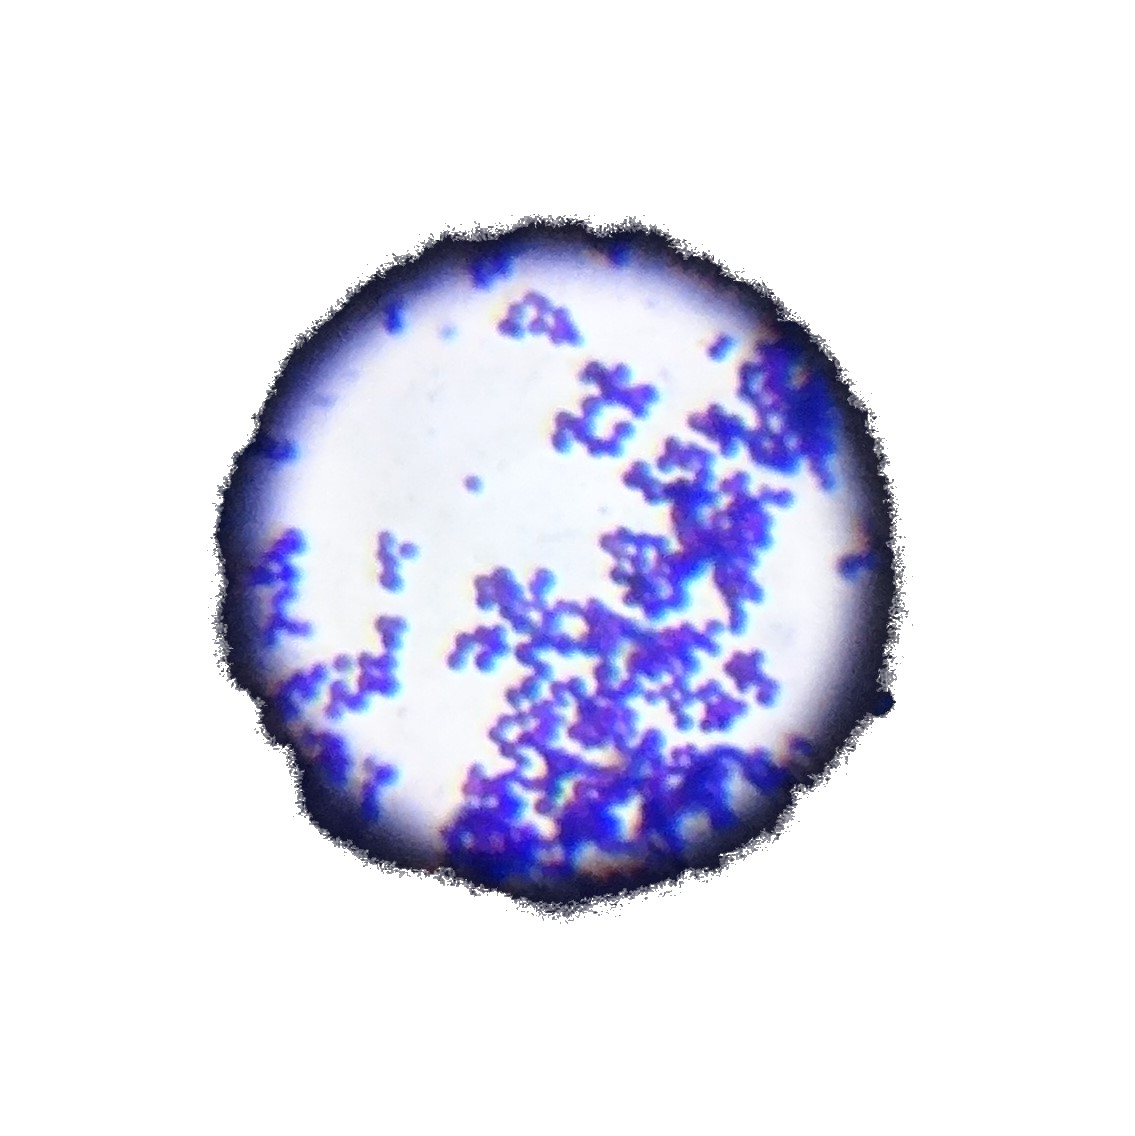
\includegraphics[width=\linewidth]{microscope.JPG}\caption{\emph{Staphylococcus aureus} as seen below the microscope. x4000, GRAM tinction}\end{subfigure}\begin{subfigure}[b]{0.4\linewidth}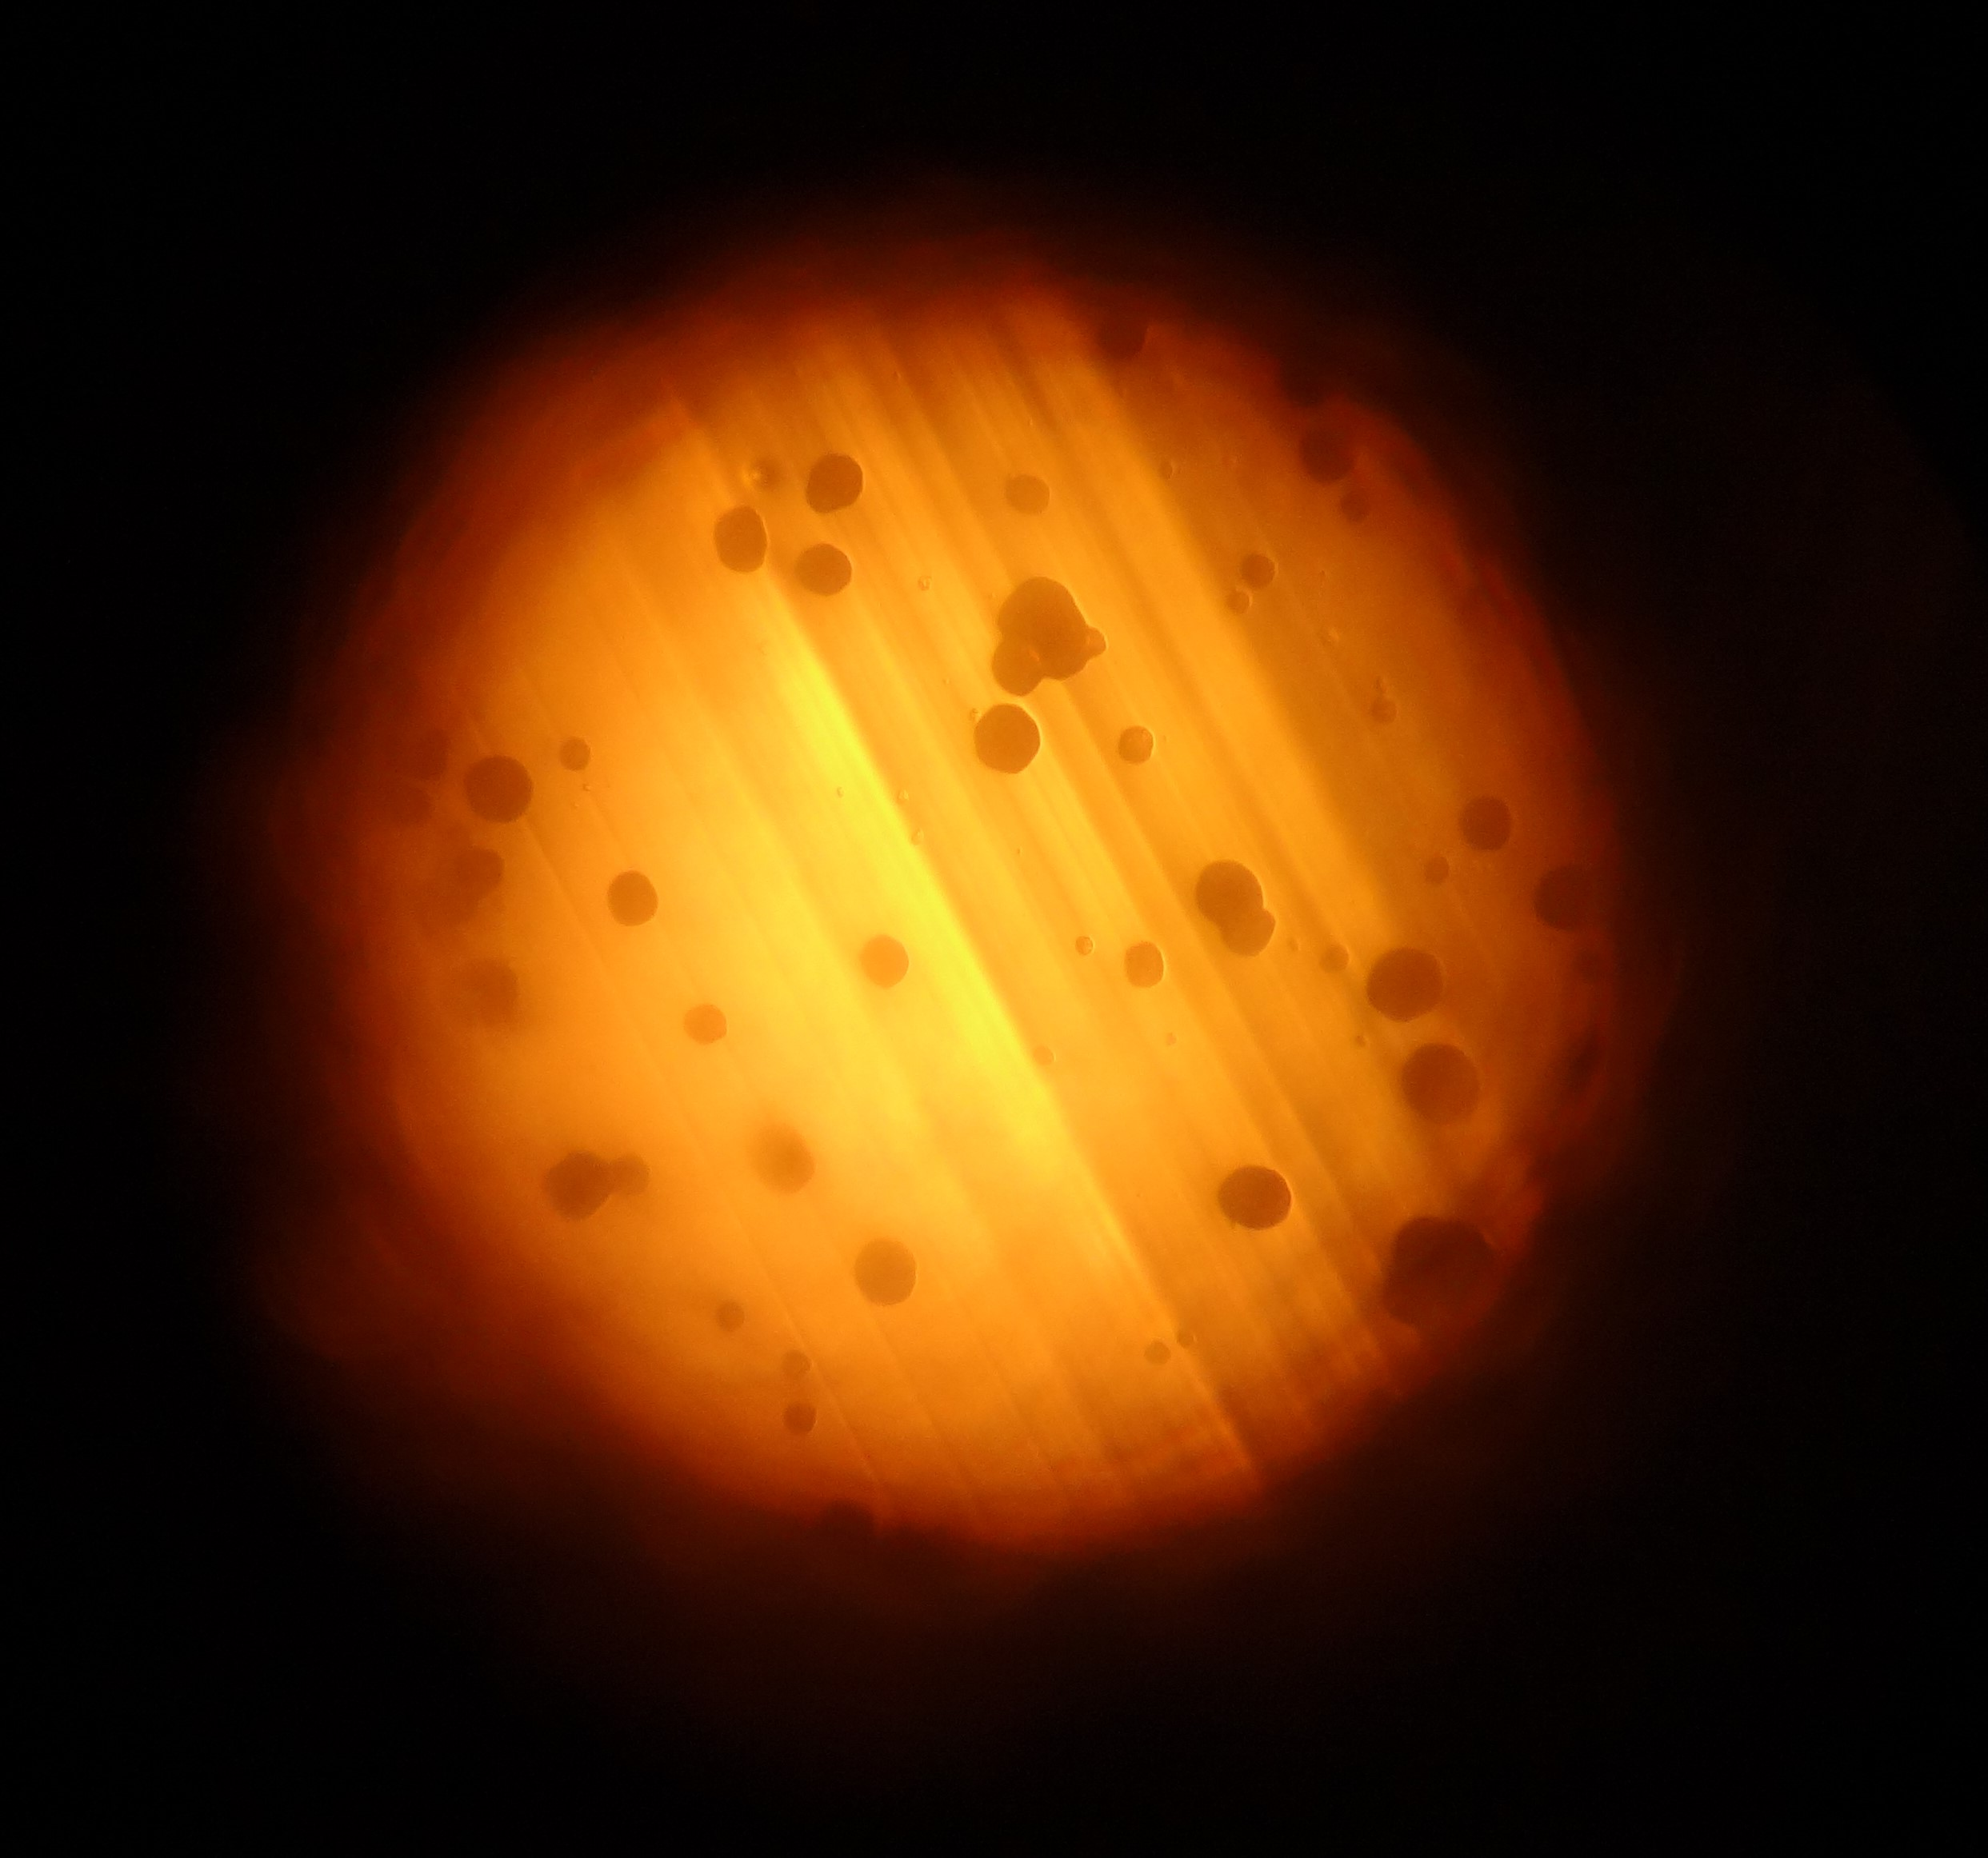
\includegraphics[width=\linewidth]{colonies.JPG}\caption{Colonies of \emph{Staphylococcus aureus} seen under a magnifying glass}\end{subfigure}\caption{Photographies of the results, as collected from my own experimentation (own data).}\end{figure}\paragraph{}There may be several reasons for the infection rate and thus natural prevalence to be increasing. One of them could be that since antibiotic abuse is growing with each passing year, the usual resident microbiota is getting killed, leaving more resources for Staph to thrive in that environment. To confirm this theory, we will look at the infection rates of a country that is facing extreme antibiotic abuse (the United States of America) and compare it to another that is controlling their antibiotics a bit better (the United Kingdom). The former have seen a 210\% increase in \emph{Staphylococcus aureus} cases since 2006. However, superfluous antibiotic prescriptions have increased by barely 1\%\cite{baggsEstimatingNationalTrends2016}. In the United Kingdom, they have seen a 160\% increase in \emph{Staphylococcus aureus} infections\cite{englandMSSABacteraemiaAnnual2021}, and their superfluous antibiotic prescriptions have gone down by 20\%. Even though this is very little data to extract conclusions from, there may be a correlation between these two factors.
\paragraph{}The other could be climate change. An increase of ambient temperatures could mean a more suitable breeding ground for this specific species and thus leading to a higher-than-usual prevalence. \emph{Staphylococcus aureus}' optimal breeding temperature is between 35\si{\celsius} and 37\si{\celsius}. The global average temperature has increased by 1,1\si{\celsius}\cite{gmsGMSAnnualGlobal2016} in the last 120 years. And \emph{Staphylococcus aureus} has a specific temperature growth curve, just like any other bacteria:\begin{figure}[H]\centering\begin{subfigure}[b]{0.4\linewidth}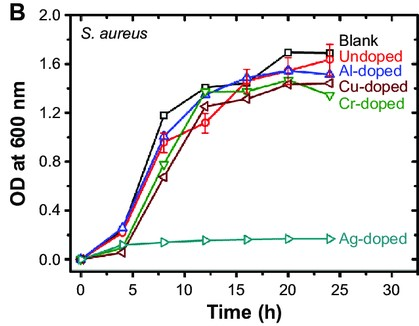
\includegraphics[width=0.95\linewidth]{tempcurve.png}\caption{\emph{Staphylococcus aureus} growth curve by temperature\cite{FigEffectTemperature2022}}\end{subfigure}\begin{subfigure}[b]{0.4\linewidth}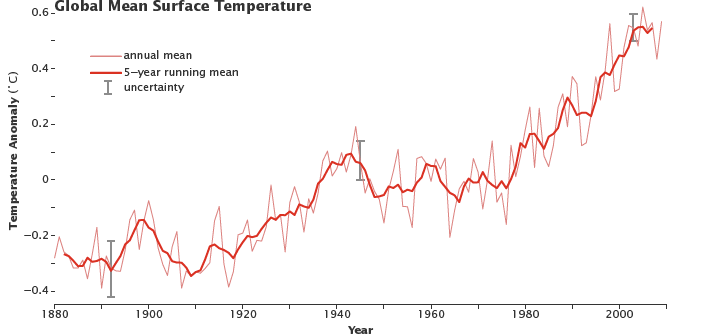
\includegraphics[width=0.95\linewidth]{warm.png}\caption{Global warming plotted by the year\cite{GlobalWarming2010}}\end{subfigure}\caption{Graphs relating the temperature of growth of \emph{Staphylococcus aureus} and the increase of temperature of the Earth.}\end{figure}So, this correlation may not be completely incorrect, and in fact some scientists warn about an increased number of infectious diseases seeing a growth in numbers due to climate change. One only data point is not enough significant data, so further study is needed on this front.

% > > > Experimental, round 2
%%----------------------------------------------------------------------------------------------------------------------------------------------------------%
\chapter{Computational experimentation}
%----------------------------------------------------------------------------------------------------------------------------------------------------------%
\epigraph{Remember that all models are wrong; the practical question is how wrong do they have to be to not be useful.}{\textit{Norman Richard Draper}}
%----------------------------------------------------------------------------------------------------------------------------------------------------------%
\section{Description}
\paragraph{}This second experiment looks at computing the shape of a \emph{Staphylococcus aureus} P-68 bacteriophage starting from its DNA sequence. This will analyze the process of protein translation, as well as looking at the process of using AlphaFold\cite{jumperHighlyAccurateProtein2021}. To compute the secondary, tertiary and quaternary structures of the proteic parts of the virus we will use the Google CoLaboratory version of AlphaFold\cite{GoogleColaboratoryAlpha1970}, as it allows for far more computer power than available on a simple laptop.
%----------------------------------------------------------------------------------------------------------------------------------------------------------%
\section{Protocol followed}
The protocol followed is very simple, as AlphaFold, the Artificial Intelligence model used does the hardest part of the work for us:
\begin{enumerate}[label=\arabic*)]
\item Convert the DNA sequence of one of the proteins to an mRNA sequence, by taking into account the fact that there's base complimentariety.
\item Convert the mRNA sequence to an aminoacid sequence of the proteins by using the genetic universal code table.
\item Feed the aminoacid sequences to AlphaFold, obtain the models for each protein.
\item Assemble the bacteriophage. 
\item Print, polish and paint a 3D physical model of the bacteriophage to illustrate better how it functions.
\end{enumerate}
The AlphaFold Jupiter notebook\cite{GoogleColaboratoryAlpha-} used is optimized for use with the NVIDIA Tesla T4 computing engine GPU, an extremely powerful graphics card, like the ones used in computers to render extremely detailed polygons in videogames or 3D animations. That's the one I used when folding\footnote{Folding a protein: calculating, by using the theorical intermolecular forces, the shape of the protein} the proteins. The genomic sequence used is NC\_004679.1, which leads to the PDB structure 6Q3G.
%----------------------------------------------------------------------------------------------------------------------------------------------------------%
\section{Results and analysis}
The gene codified for a total of 22 separate proteins. After BLASTing\footnote{BLAST: digital service that takes a sequence of DNA in the FASTA format and attempts to find the organism and/or protein that it codifies} all of them, I got the following list:
\begin{center}\begin{figure}[H]\centering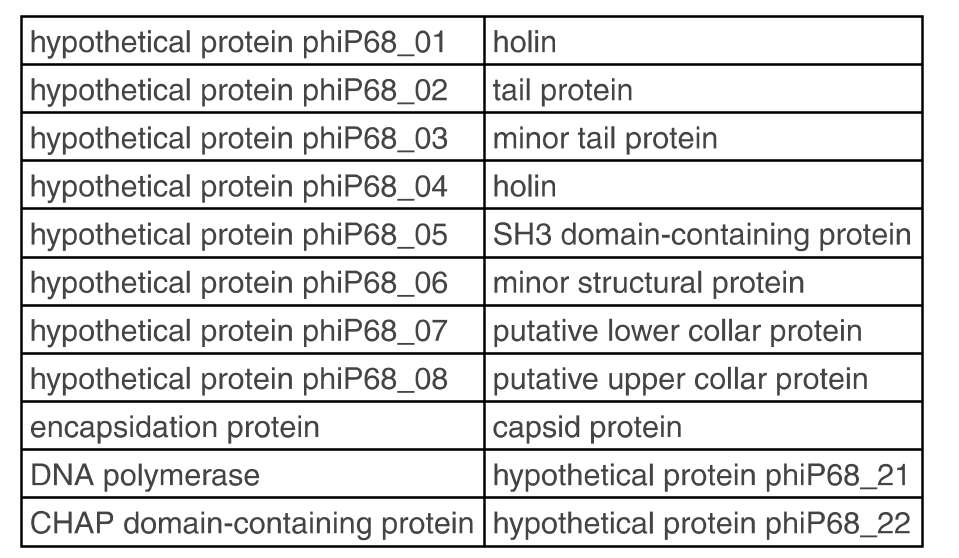
\includegraphics[width=0.90\textwidth]{AF3.png}\end{figure}\end{center}
Which then assembled into the following figure:
\begin{center}\begin{figure}[H]\centering\includegraphics[width=0.90\textwidth]{p68.png}\end{figure}\end{center}
These three views allow us to see the capsid, the collar and sheath, the tail fibers, and the spikes, which are integrated into the collar. The tail fibers act exactly like the Coronavirus spike proteins: they bind to a specific compound on the surface of the bacteria, but they don't access it. They only bind to the surface, perforate it using the spikes and then, due to a difference in pressures, the genetic material is expulsed into the cell. Then, it uses the fact that bacteria will integrate strands of genetic material floating in the environment into its own hereditary material in order to force the host to reproduce the virus.
\paragraph{}Using the PDB2STL pymol\footnote{Pymol: program that takes a protein database and converts it into a viewable model} tool, I managed to create a printable 3D model of the virus, which was then polished using a wire brush and painted gray so the details can be seen with more clarity. Then, a white filament strand was added to symbolize the genetic material being oozed into a cell:
\begin{center}\begin{figure}[H]\centering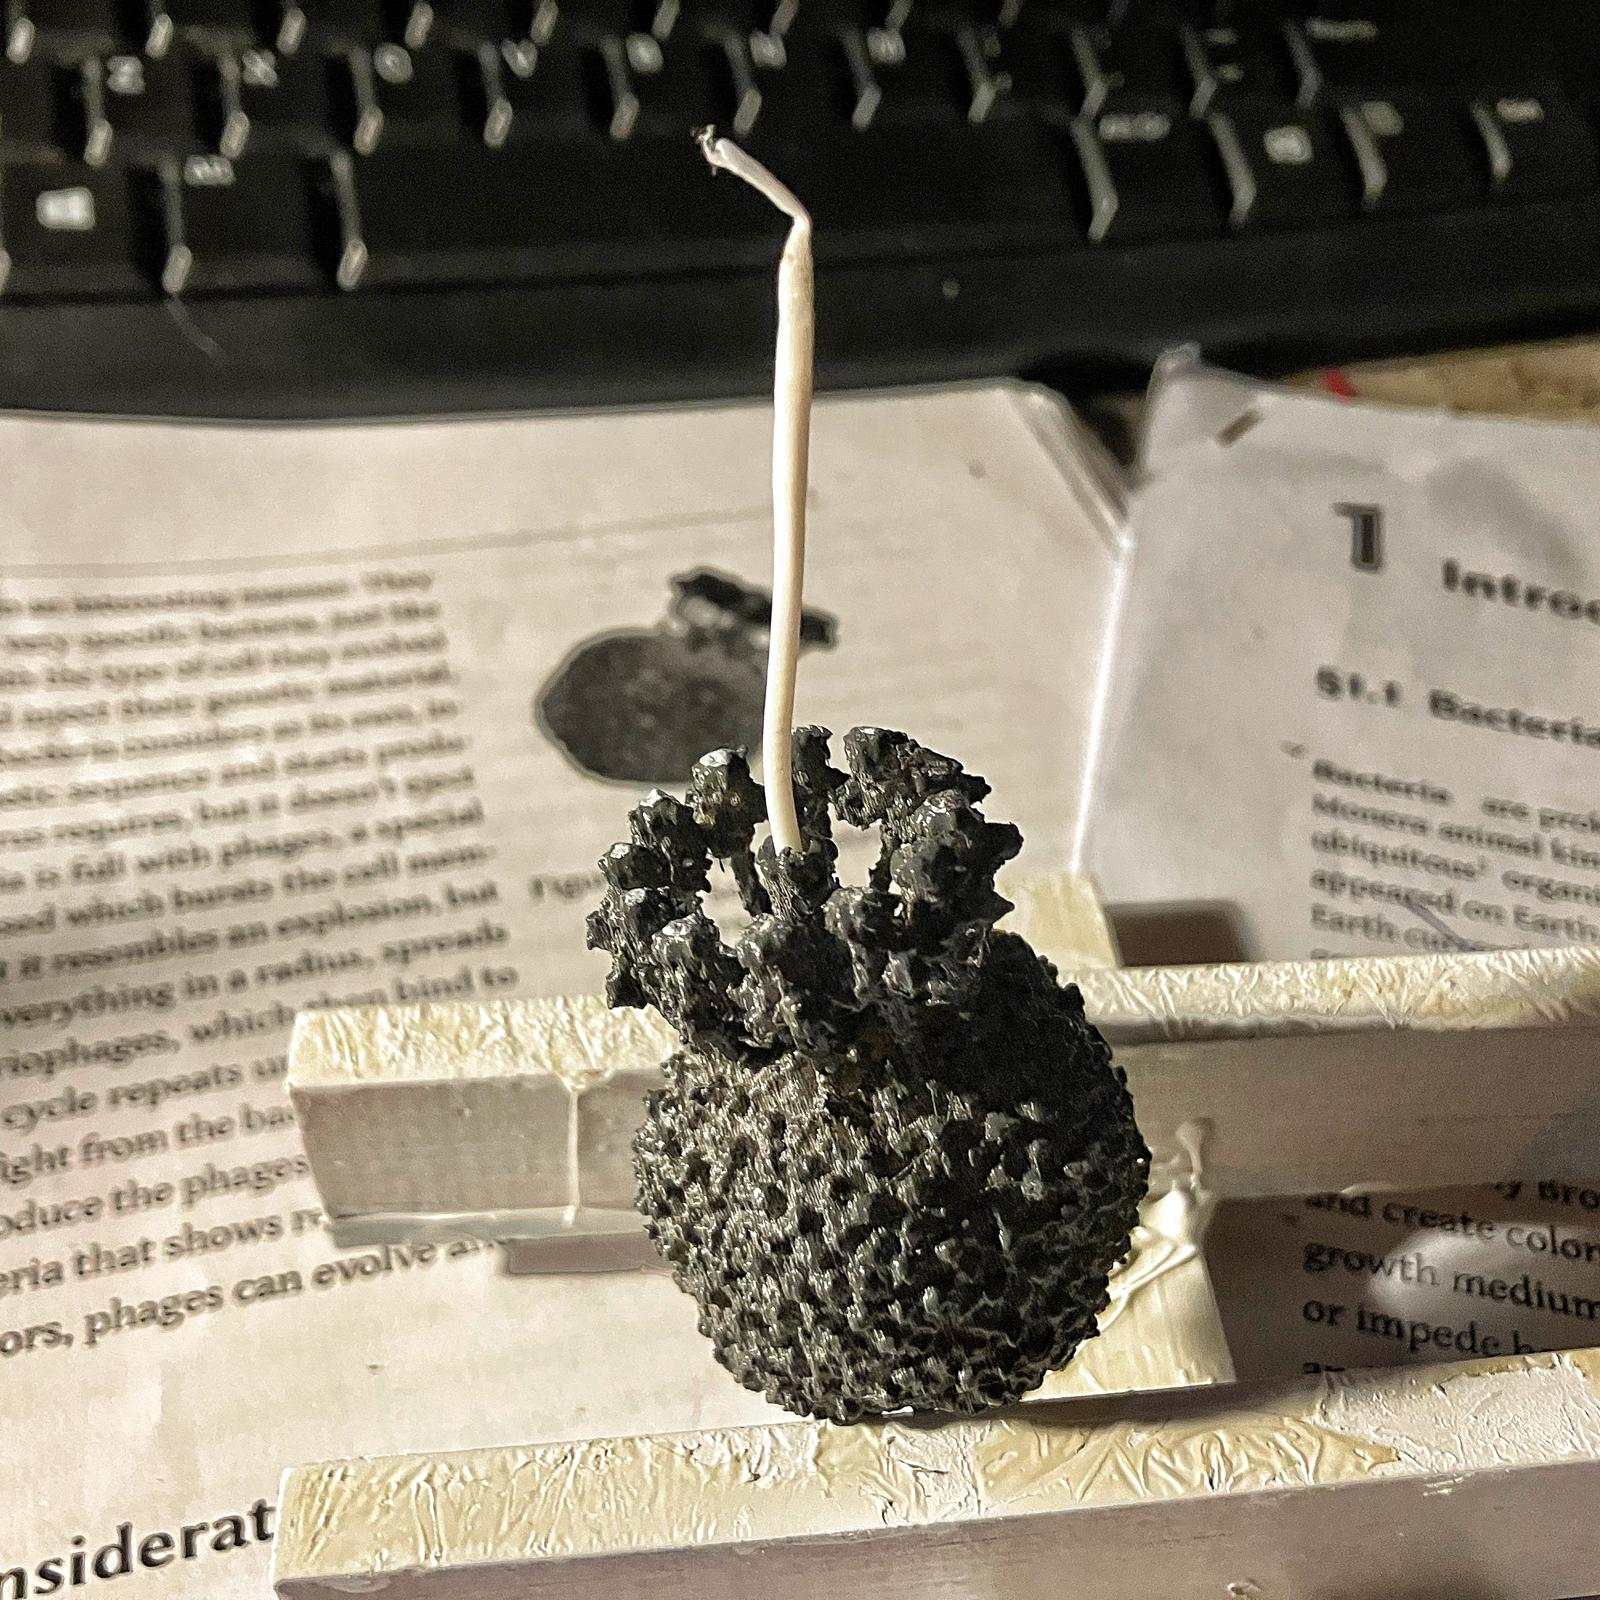
\includegraphics[width=0.50\textwidth]{3dirl.jpg}\end{figure}\end{center}
% > > > Theorem Environments
%%=-=-=-=-=-=-=-=-=-=-=-=-=-=-=-=-=-=-=-=-=-=-=-=-=-=-=-=-=-=-=-=-=-=- CHAPTER 03
\chapter{Theorem Environments}

%=-=-=-=-=-=-=-=-=-=-=-=-=-=-=-=-=-=-=-=-=-=-=-=-=-=-=-=-=-=-=-=-=-=-=-= SECTION
\section{Definition}

%=-=-=-=-=-=-=-=-=-=-=-=-=-=-=-=-=-=-=-=-=-=-=-=-=-=-=-=-=-=-=-==-=-= DEFINITION
\begin{definition}[Definition Of Subtraction]
\label{0000}\index{Definition!0000}
Given \( a \) and \( b \) are real numbers, then
\cite{Olson2021}
\begin{align*}
    a + (-b) &= a - b.
\end{align*}
\end{definition}
%=-=-=-=-=-=-=-=-=-=-=-=-=-=-=-=-=-=-=-=-=-=-=-=-=-=-=-=-=-=-=-=- END DEFINITION

%=-=-=-=-=-=-=-=-=-=-=-=-=-=-=-=-=-=-=-=-=-=-=-=-=-=-=-=-=-=-=-=-=-=-=-= SECTION
\section{Examples}

%=-=-=-=-=-=-=-=-=-=-=-=-=-=-=-=-=-=-=-=-=-=-=-=-=-=-=-=-=-=-=-=-=-=-=-= EXAMPLE
\begin{example}
\label{0001}\index{Example!0001}
Solve the equation \( x + 4 = 7 \) for all \( x \in \setZ \).
\end{example}
% solution
\begin{solution}
The solution set is \( x = \set{3} \).
\end{solution}
%=-=-=-=-=-=-=-=-=-=-=-=-=-=-=-=-=-=-=-=-=-=-=-=-=-=-=-=-=-=-=-=-=-= END EXAMPLE

%=-=-=-=-=-=-=-=-=-=-=-=-=-=-=-=-=-=-=-=-=-=-=-=-=-=-=-=-=-=-=-=-=-=-=-= SECTION
\section{Theorems}

%=-=-=-=-=-=-=-=-=-=-=-=-=-=-=-=-=-=-=-=-=-=-=-=-=-=-=-=-=-=-=-==-=-=-=-=- AXIOM
\begin{axiom}[Axiom Of Simple Mathematical Induction]
\label{0005}\index{axiom!0005}
Let \(P(n)\) be a proposition, where \( n \in \setZp \) .  If we can
\begin{enumerate}
    \item show the basis step is TRUE by showing \(P(1)\) is TRUE and 
    \item show the inductive step is TRUE by showing for each 
    \( r \in \setZp \), whenever \( P(r) \) is TRUE , then \( P(r + 1) \) is
    TRUE, where \( P(r) \) is called the \defw{induction hypothesis}, 
\end{enumerate}
then by the \defw{axiom of mathematical induction} the proposition is proved.
        
The axiom of simple mathematical induction cannot be proven as it is part of the definition of \(\setZp\).
        
\end{axiom}
%=-=-=-=-=-=-=-=-=-=-=-=-=-=-=-=-=-=-=-=-=-=-=-=-=-=-=-=-=-=-=-==-=-=- END AXIOM

The axiom of simple mathematical induction\ref{0005} cannot be proven as it is 
included as part of the definition of the set of positive integers, 
\( \setZp \).

%=-=-=-=-=-=-=-=-=-=-=-=-=-=-=-=-=-=-=-=-=-=-=-=-=-=-=-=-=-=-=-==-=- PROPOSITION
\begin{proposition}[Product of Common Base Powers]
\label{0003}\index{Proposition!0003}
Given \( b^m \) and \( b^n \), then
\begin{align*}
    b^m \cdot b^n &= b^{m + n}.
\end{align*}
\end{proposition}
\begin{proof}
    Coming Soon!
\end{proof}
%=-=-=-=-=-=-=-=-=-=-=-=-=-=-=-=-=-=-=-=-=-=-=-=-=-=-=-=-=-=-=-= END PROPOSITION

%=-=-=-=-=-=-=-=-=-=-=-=-=-=-=-=-=-=-=-=-=-=-=-=-=-=-=-=-=-=-=-==-=- PROPOSITION
\begin{theorem}[Pythagorean Theorem]
    \label{0004}\index{Theorem!0004}
    Given a right-angled triangle \( ABC \) with sides \( a, b \) and \( c \),
    where \( c \) is the hypotenuse, then
    \begin{align*}
        a^2 + b^2 &= c^2.
    \end{align*}
    \end{theorem}
    \begin{proof}
        Someday soon!
    \end{proof}
%=-=-=-=-=-=-=-=-=-=-=-=-=-=-=-=-=-=-=-=-=-=-=-=-=-=-=-=-=-=-=- END PROPOSITION


% > > > Works Cited
%%=-=-=-=-=-=-=-=-=-=-=-=-=-=-=-=-=-=-=-=-=-=-=-=-=-=-=-=-=-=-=-=-=-=- CHAPTER 03
\chapter{Works Cited}


% > > > What is LaTeX
%%=-=-=-=-=-=-=-=-=-=-=-=-=-=-=-=-=-=-=-=-=-=-=-=-=-=-=-=-=-=-=-=-=-=- CHAPTER 06
\chapter{What is \LaTeX?}

% =-=-=-=-=-=-=-=-=-=-=-=-=-=-=-=-=-=-=-=-=-=-=-=-=-=-=-=-=-=-=-=-=-=-= SECTION
\section{A Brief History of \TeX}

The programming language \TeX\ was created by Donald Knuth in the late
1970s to typeset beautifully formatted documents that could be easily published
using a computer without having to go through professionals typesetters.
Knuth was trying to solve the problem of having to bring unformatted writing,
called a manuscript, to a typesetter where they would decide how to best format
your work by deciding things such as the font, how to space the characters on a
line and where to place images. Imagine how stressed you would feel sending off
a piece of IB coursework to be typeset and then have it returned in a form
that did not meet your expectations and being forced to sent that published
work to be graded.

Today, desktop publishing has never been easier with options such as Microsoft
Word and Google Documents.  So why has \TeX\ remained the standard in the
mathematics and scientific community for writing and publishing documents?
With these applications being easy to use, there must be some compelling
reasons to invest in learning a computer language that has a steep learning
curve.

As you probably guessed, the typesetter probably will not format your document 
exactly how you envisioned it to be.  You can imagine the frustration of having 
to give feedback on the document produced by the typesetter and then wait for their 
modifications. 

the automate the process of formatting text ready for publication, 
a process called typesetting.  It seems that Knuth was inspired to take control
of the typesetting process in 1974 when he stopped sending his work
the the American Mathematics Society because \textquote[{\cite{FoRKArchiveBrief}}]{the finished
product was just too painful for me to look at}.  On May 13, 1977, Knuth 
shares a description of his preliminary vision of how \TeX\ will work to automate 
automate the process of formatting text ready for publication

It worked by the user creating a \texttt{foo.tex} 
text file formatted with commands collectively called plain\TeX\. This file would 
then be interpreted by a computer program called the \TeX\ engine, which would 
output a device independent file, \texttt{foo.dvi}, that could be sent to printer or 
converted to another file format such as \texttt{foo.ps} or \texttt{foo.pdf}.
%=-=-=-=-=-=-=-=-=-=-=-=-=-=-=-=-=-=-=-=-=-=-=-=-=-=-=-=-=-=-=-=-=-=- DEFINITION
\begin{definition}[Engine]
\label{defn:engine}\index{Definition!Engine}
An \defw{engine} is a computer program that \defw{compiles} one or more input 
files written using a programming language to produce a output file.
\end{definition}
%=-=-=-=-=-=-=-=-=-=-=-=-=-=-=-=-=-=-=-=-=-=-=-=-=-=-=-=-=-=-=-=- END DEFINITION

% =-=-=-=-=-=-=-=-=-=-=-=-=-=-=-=-=-=-=-=-=-=-=-=-=-=-=-=-=-=-=-=-=-=-= SECTION
\section{A Brief History of \TeX}


%----------------------------------------------------------------------------------------------------------------------------------------------------------%
\backmatter\renewcommand{\thepage}{\roman{page}}\setcounter{page}{0}

\clearpage
\printbibliography[title={References}]
\cleardoublepage\part{Appendix}\appendix
\chapter{Annex 1 - Protocol as published in protocols.io}
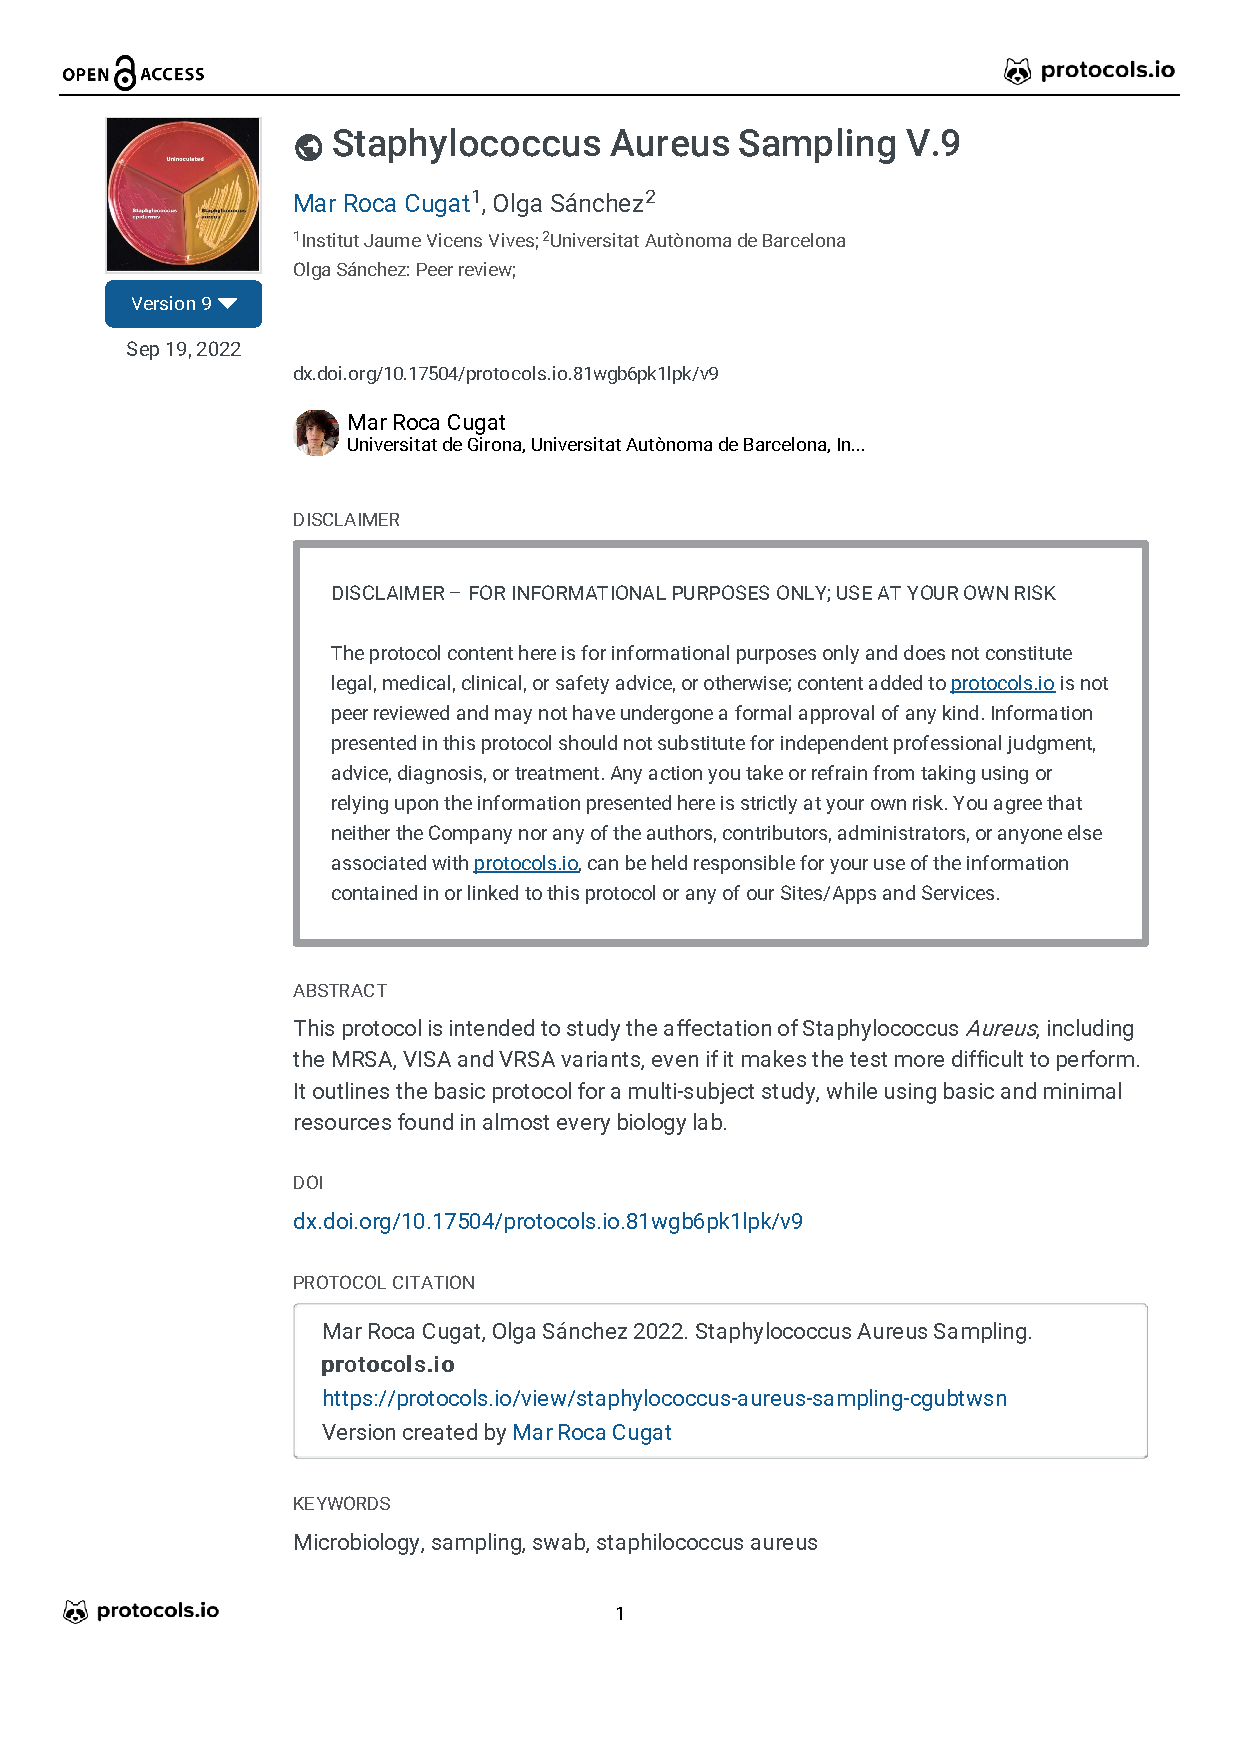
\includepdf[pages=-]{protocol.pdf}
%\include{chapters/somechapter}
\end{document}